\chapter{Experiment and Results}\label{ch:5}

\section{Evaluation}

\subsection{Evaluation Targets}

In the proposed framework, there are several components we have to evaluate in order to answer our research questions.
The following list explains the targets to evaluate, and Figure 5.1 indicates where the targets are located in our proposed framework.

\begin{quote}
  \begin{itemize}
    \item T1: Motivation to access the campus by location-based AR contents
    \item T2: Motivation to access the campus by co-creation process
    \item T3: Motivation to access the campus by interaction between users
    \item T4: Changes in the image of the campus by location-based AR contents
    \item T5: Changes in the image of the campus by co-creation process
    \item T6: Changes in the image of the campus by interaction between users
  \end{itemize}
\end{quote}

\begin{figure}[ht]
  \centering
  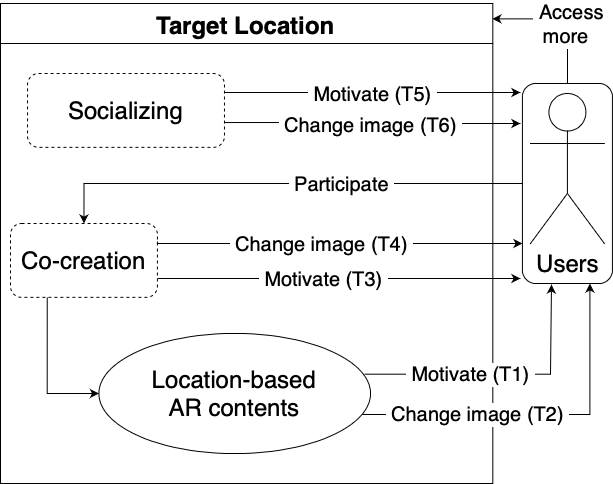
\includegraphics[width=0.8\columnwidth]{resources/5_experiment_and_results/proposed_framework_with_validate_targets.png}
    \caption{Proposed framework and targets to evaluate}
\end{figure}

\subsection{Evaluation of Motivation}

To evaluate targets about motivation, including T1, T2 and T3, we adopted questions from Situational Motivation Scale (SIMS) \cite{guay_vallerand_blanchard_2000} for measurement.
SIMS contains four categories of motivation: 'Intrinsic motivation', 'Extrinsic motivation', and 'Amotivation', while in this study we specifically adopted 'Intrinsic motivation (IM)' and 'Amotivation (AM)'.
'Extrinsic motivation', including 'Identified regulation (IR)' and 'External regulation (ER)' are excluded since what we wanted to measure is the motivation induced by components in the proposed framwork, instead of following any instruction, obiligation, or any other external factors.
Questions we adopted from SIMS are listed in Appendix A.
Here we adopted 6 point scales to avoid ambiguous responses (where users keep choosing the middle item).

Cahyono et al. adopted SIMS with the use of Self-Determination Index (SDI) for scoring, which is calculated by the formula below:
\[ SDI = (2 * IM) + IR - ER - (2 * AM) \]
The higher the value of SDI, the more intrinsically motivated a person is \cite{cahyono_ludwig_2017}.
However, since we excluded IR and ER in this study, we conducted the scoring with:

\[ IM - AM \]

and composed hypotheses for the scoring of motivation, listed below: 

\begin{quote}
  \begin{itemize}
    \item H1: For T1, the value of IM - AM measured with SIMS is positive.
    \item H2: For T2, the value of IM - AM measured with SIMS is positive.
    \item H3: For T3, the value of IM - AM measured with SIMS is positive.
  \end{itemize}
\end{quote}

Besides the scales, we also prepared questions for free comments about motivation.

\subsection{Evaluation of Changes in the Image of the Campus}

To evaluate targets about changes in the image of the campus, including T4, T5 and T6,
we prepared a question with 5 point scale, described as follows:

\begin{quote}
  Does the image of campus in your mind changed?
  \begin{enumerate}
    \item Not at all
    \item Only a little
    \item Somehow changed
    \item Changed a lot
    \item Completely changed
  \end{enumerate}
\end{quote}

Besides the scales, we also prepared questions for free comments about changes in the image of the campus.

\subsection{Questionnaires}

Then we designed 4 questionnaires prepared for participants in an experiment conducted later (explanation in section 5.2). Each questionnaire corresponds to a topic listed as follows:

\begin{quote}
  \begin{enumerate}
    \item Viewing location-based AR contents, the graffiti, in the campus
    \item Creating location-based AR contents, the graffiti, in the campus
    \item Interactions with other users
    \item Overall experience of using the prototype
  \end{enumerate}
\end{quote}

In each questionnaire, we asked questions about how the experience of the topic during the experiment affected one's motivation to access the campus, with questions introduced in Section 5.1.2, as well as changes in the image of the campus in one's mind, with questions introduced in Section 5.1.3.
For example, Questionnaire 1 includes questions about the motivation and changes in the image of the campus influenced by the experience of viewing location-based AR contents in the campus.

Results from Questionnaire 1 correspond to the evaluation of T1 and T4, Questionnaire 2 to T2 and T5, Questionnaire 3 to T3 and T6, and finally Questionnaire 4 to the whole framwork.
% In Questionnaire 1, 2 and 4, we also asked questions about participants' feeling of presence to check its relevance to the questionnaire's topic.
In Questionnaire 3, we also included questions about awareness of other users' existence and interaction with them.
Eventually, in each questionnaire, we also asked whether a participant, after attending the experiment, prefers our location-based AR prototype or a similar one without location-based features and AR effect but usable at home,
in order to make clear of the importance of location-based AR.

\section{Experiment}

At first, we conducted a preliminary survey with 3 participants trying the prototype in Waseda University Nishi-Waseda Campus for one week.
3 participants gave us positive responses about their motivation to access campus after experiencing the prototype.
We also improved the app based on their feedbacks, such as adding features that allow users to review/edit/delete their own graffiti.
The experinemt lasted for 2 weeks. 14 males and 2 females participated,
and they are asked to use the prototype freely in the same campus at least twice a week.
Before the experiment, we asked participants about their frequencies of accessing the campus and the images of campus in their mind before and after the pandemic started spreading,
in order to understand how much impact the pandemic brought on each participant.
Instruction of using the prototype was also distributed before the experiment.
2 weeks later, after the experiment finished, participants were required to answer the questionnaires introduced in Section 5.1.

We also conducted a control experiment, with 3 males and 1 females participating in playing a similar prototype without location-based features and AR effect but usable at home for a week.
Then we asked them to fill in the same questionnaires.

\section{Results}
\subsection{Motivations}

\begin{table}[h]
  \begin{tabular}{l || R{4cm} | R{3cm} | R{2.5cm}}
    \hline
    \rowcolor{lightgray}
          & \multicolumn{1}{c |}{Intrinsic motivation (IM)} & \multicolumn{1}{c |}{Amotivation (AM)} & \multicolumn{1}{c}{IM - AM}  \\
    \hline
    Mean   & 4.3906 & 2.7500 & 1.6406  \\
    Median & 4.3750 & 3.0000 & 1.6250  \\
    Min    & 3.0000 & 1.0000 & -1.5000 \\
    Max    & 6.0000 & 4.5000 & 5.0000  \\
    SD     & 0.7636 & 1.0124 & 1.5916  \\
    \hline
  \end{tabular}
  \caption{Motivation to access campus influenced by viewing location-based AR contents}
    \label{table:1}
\end{table}

\begin{table}[h]
  \begin{tabular}{l || R{4cm} | R{3cm} | R{2.5cm}}
    \hline
    \rowcolor{lightgray}
          & \multicolumn{1}{c |}{Intrinsic motivation (IM)} & \multicolumn{1}{c |}{Amotivation (AM)} & \multicolumn{1}{c}{IM - AM}  \\
    \hline
    Mean   & 4.4833 & 2.5167 & 1.9667  \\
    Median & 4.2500 & 2.5000 & 2.0000  \\
    Min    & 3.0000 & 1.0000 & -1.5000 \\
    Max    & 6.0000 & 4.5000 & 5.0000  \\
    SD     & 0.8044 & 1.0021 & 1.6767  \\
    \hline
  \end{tabular}
  \caption{Motivation to access campus influenced by participation in co-creation}
    \label{table:2}
\end{table}

\begin{table}[h]
  \begin{tabular}{l || R{4cm} | R{3cm} | R{2.5cm}}
    \hline
    \rowcolor{lightgray}
          & \multicolumn{1}{c |}{Intrinsic motivation (IM)} & \multicolumn{1}{c |}{Amotivation (AM)} & \multicolumn{1}{c}{IM - AM}  \\
    \hline
    Mean   & 4.3833 & 2.5833 & 1.7200  \\
    Median & 4.7500 & 2.0000 & 1.8000  \\
    Min    & 2.0000 & 1.0000 & -2.0000 \\
    Max    & 6.0000 & 5.0000 & 5.0000  \\
    SD     & 1.1135 & 1.1286 & 2.0743  \\
    \hline
  \end{tabular}
  \caption{Motivation to access campus influenced by interaction with other users}
    \label{table:3}
\end{table}

\begin{table}[h]
  \begin{tabular}{l || R{4cm} | R{3cm} | R{2.5cm}}
    \hline
    \rowcolor{lightgray}
          & \multicolumn{1}{c |}{Intrinsic motivation (IM)} & \multicolumn{1}{c |}{Amotivation (AM)} & \multicolumn{1}{c}{IM - AM}  \\
    \hline
    Mean   & 4.5469 & 2.5313 & 2.0156  \\
    Median & 4.6250 & 2.2500 & 2.6250  \\
    Min    & 3.0000 & 1.0000 & -2.0000 \\
    Max    & 6.0000 & 5.0000 & 5.0000  \\
    SD     & 0.8328 & 1.0950 & 1.8108  \\
    \hline
  \end{tabular}
  \caption{Motivation to access campus influenced by overall experience of the prototype}
    \label{table:4}
\end{table}

\subsection{Image of Campus}

\begin{table}[h]
  \begin{tabular}{l || R{3.5cm} | R{2.5cm} | R{2cm} | R{2cm}}
    \hline
    \rowcolor{lightgray}
          & \multicolumn{1}{C{3.5cm} |}{Viewing location- \newline based AR contents} & \multicolumn{1}{C{2.5cm} |}{Participation \newline in co-creation} & \multicolumn{1}{C{2cm} |}{User-user \newline interaction} & \multicolumn{1}{C{2cm}}{Overall \newline experience} \\
    \hline
    Mean   & 2.6875 & 2.7333 & 2.8667 & 2.8750 \\
    Median & 3.0000 & 3.0000 & 3.0000 & 3.0000 \\
    Min    & 2.0000 & 2.0000 & 2.0000 & 2.0000 \\
    Max    & 4.0000 & 4.0000 & 4.0000 & 4.0000 \\
    SD     & 0.6021 & 0.5936 & 0.8338 & 0.8062 \\
    \hline
  \end{tabular}
  \caption{Changes in the image of the campus, scaled from 1 (Not at all) to 5 (Completely changed)}
    \label{table:5}
\end{table}

\subsection{User-user Interaction}

\begin{table}[h]
  \begin{tabular}{l || R{5cm} | R{5.5cm}}
    \hline
    \rowcolor{lightgray}
          & \multicolumn{1}{C{5cm} |}{I felt existence \newline of other users} & \multicolumn{1}{C{5.5cm}}{It felt like I am \newline interacting with other users} \\
    \hline
    Mean   & 4.5333 & 4.0000 \\
    Median & 5.0000 & 4.0000 \\
    Min    & 3.0000 & 2.0000 \\
    Max    & 6.0000 & 6.0000 \\
    SD     & 0.9155 & 1.3093 \\
    \hline
  \end{tabular}
  \caption{Sense of other users' existence and interaction, scaled from 1 (Disagree) to 6 (Agree)}
    \label{table:6}
\end{table}

% \subsection{Revelance of Feeling of Presence}

\subsection{Comparison with cases without location-based AR features}

\begin{table}[h]
  \begin{tabular}{l || R{3.5cm} | R{2.5cm} | R{2cm} | R{2cm}}
    \hline
    \rowcolor{lightgray}
          & \multicolumn{1}{C{3.5cm} |}{Viewing location- \newline based AR contents} & \multicolumn{1}{C{2.5cm} |}{Participation \newline in co-creation} & \multicolumn{1}{C{2cm} |}{User-user \newline interaction} & \multicolumn{1}{C{2cm}}{Overall \newline experience} \\
    \hline
    Mean   & 4.8125 & 4.8667 & 4.6000 & 4.7500 \\
    Median & 5.0000 & 6.0000 & 5.0000 & 6.0000 \\
    Min    & 1.0000 & 1.0000 & 1.0000 & 1.0000 \\
    Max    & 7.0000 & 7.0000 & 7.0000 & 7.0000 \\
    SD     & 1.6419 & 1.8074 & 1.6388 & 1.8074 \\
    \hline
  \end{tabular}
  \caption{Preference between prototype at campus or prototype at home, scaled from 1 (At home) from 7 (At campus)}
    \label{table:7}
\end{table}
